% !TeX document-id = {95a8edac-103b-4a15-9950-88e55882fea3}
% !TeX program = xelatex

\documentclass[aspectratio=169,xcolor={dvipsnames}
%,notes=only
%,notes
%,show notes on second screen=right
,handout
]{beamer}
\usetheme[background=light, numbering=fraction]{metropolis}
\usepackage{appendixnumberbeamer}
\usepackage{pgfpages}

\usepackage{FiraMono}

\setmonofont[
Scale=MatchLowercase,
Contextuals={Alternate}
]{Fira Mono}

\usepackage[newfloat,cache=false]{minted}
% \usemintedstyle{autumn}
\usemintedstyle{tango}

\setminted[rust]{obeytabs=true,tabsize=2}

\usepackage{twemojis}

% Helpful defines
\newcommand{\ourtech}{\textsc{Galette}}
\newcommand{\afxdp}{\texttt{AF\_XDP}}
\newcommand{\af}{(\texttt{AF\_})XDP}
\newcommand{\afp}{\texttt{AF\_PACKET}}

% You will need to modify these, the authors down below,
% and likely the \addbibresource statements below.
\newcommand{\mytitle}{\ourtech:~a~Lightweight~XDP~Dataplane on~your~Raspberry~Pi}
\newcommand{\myemail}{kylesimpson1@acm.org}
\newcommand{\myurl}{https://mcfelix.me}
\newcommand{\mygithub}{FelixMcFelix}

%\usepackage[T1]{fontenc}

\usepackage{bm}
\usepackage{mathtools}

\usepackage[labelfont=bf,textfont={it}]{caption}
\usepackage{subcaption}
\captionsetup[figure]{justification=centering}
\captionsetup[subfigure]{justification=centering}

\usepackage{tikz}
\usepackage{varwidth}
\usetikzlibrary{arrows.meta, calc, fit, positioning, shapes}

\usepackage[title]{appendix}

\usepackage{etoolbox}
\usepackage[per-mode=symbol]{siunitx}
\robustify\bfseries
\robustify\emph
%\robustify\uline
\sisetup{detect-all, range-phrase=--, range-units=single, detect-weight=true, table-format=1.3}
\DeclareSIUnit{\packet}{p}

\usepackage[siunitx]{circuitikz}

%\usepackage{fontspec}
%\setsansfont{Fira Sans Mono}

\usepackage[UKenglish]{babel}
\usepackage{csquotes}

\usepackage{amssymb}

\usepackage{lipsum}
%\usepackage[basic]{complexity}
\usepackage[super,negative]{nth}

\usepackage{booktabs}

%bib
\usepackage[maxnames=3,maxbibnames=99,mincrossrefs=5,sortcites
%,backend=bibtex
,style=authortitle
]{biblatex}
\addbibresource{bibliography.bib}

% official colours
\definecolor{uofguniversityblue}{rgb}{0, 0.219608, 0.396078}

\definecolor{uofgheather}{rgb}{0.356863, 0.32549, 0.490196}
\definecolor{uofgaquamarine}{rgb}{0.603922, 0.72549, 0.678431}
\definecolor{uofgslate}{rgb}{0.309804, 0.34902, 0.380392}
\definecolor{uofgrose}{rgb}{0.823529, 0.470588, 0.709804}
\definecolor{uofgmocha}{rgb}{0.709804, 0.564706, 0.47451}

\definecolor{uofglawn}{rgb}{0.517647, 0.741176, 0}
\definecolor{uofgcobalt}{rgb}{0, 0.615686, 0.92549}
\definecolor{uofgturquoise}{rgb}{0, 0.709804, 0.819608}
\definecolor{uofgsunshine}{rgb}{1.0, 0.862745, 0.211765}
\definecolor{uofgpumpkin}{rgb}{1.0, 0.72549, 0.282353}
\definecolor{uofgthistle}{rgb}{0.584314, 0.070588, 0.447059}
\definecolor{uofgpillarbox}{rgb}{0.701961, 0.047059, 0}
\definecolor{uofglavendar}{rgb}{0.356863, 0.301961, 0.580392}

\definecolor{uofgsandstone}{rgb}{0.321569, 0.278431, 0.231373}
\definecolor{uofgforest}{rgb}{0, 0.317647, 0.2}
\definecolor{uofgburgundy}{rgb}{0.490196, 0.133333, 0.223529}
\definecolor{uofgrust}{rgb}{0.603922, 0.227451, 0.023529}

\definecolor{inferno0}{rgb}{0.001462 0.000466 0.013866}
\definecolor{inferno64}{rgb}{0.341500 0.062325 0.429425}
\definecolor{inferno128}{rgb}{0.735683 0.215906 0.330245}
\definecolor{inferno192}{rgb}{0.978422 0.557937 0.034931}
\definecolor{inferno255}{rgb}{0.988362 0.998364 0.644924}

%picky abt et al.
\usepackage{xpatch}

\makeatletter\let\expandableinput\@@input\makeatother

\xpatchbibmacro{name:andothers}{%
	\bibstring{andothers}%
}{%
	\bibstring[\emph]{andothers}%
}{}{}

%opening!

\usepackage{cleveref}
\newcommand{\crefrangeconjunction}{--}

\usepackage{fontawesome5}

\addtobeamertemplate{footnote}{\vspace{-6pt}\advance\hsize-0.5cm}{\vspace{6pt}}
\makeatletter
% Alternative A: footnote rule
\renewcommand*{\footnoterule}{\kern -3pt \hrule \@width 2in \kern 8.6pt}
% Alternative B: no footnote rule
% \renewcommand*{\footnoterule}{\kern 6pt}
\makeatother

\usepackage[export]{adjustbox}
\usetikzlibrary{arrows.meta, calc, fit, positioning, shapes.misc}

% \expandableinput is useful for some tables etc.
\makeatletter\let\expandableinput\@@input\makeatother
\newcommand{\cmark}{\ding{51}}%
\newcommand{\xmark}{\ding{55}}%

%-------------------------------------%
%-------------------------------------%

\title{\mytitle}
\author{\vspace{-1em}\textbf{Kyle A.\ Simpson}, Chris Williamson, Douglas J.\ Paul, Dimitrios P.\ Pezaros\\
	\faEnvelopeOpen{} \href{mailto:\myemail}{\nolinkurl{\myemail}}\\
	\vspace{1em}\small{\faGithub{} \href{https://github.com/\mygithub}{\mygithub} \hspace{0.5em} \faGlobe{} \url{\myurl}}}
\institute{University of Glasgow}
\date{13th June, 2023}

\begin{document}
% title fun, including Org logos....
\begin{frame}
	\maketitle
	\begin{tikzpicture}[overlay, remember picture]
%		\node[above right=0.8cm and 0.9cm of current page.south west] (esnet-logo) {
\includegraphics[width=2.75cm]{netlab-trim}};
%		\node[right=1cm of esnet-logo] {\adjincludegraphics[height=2cm,trim={0 {.4\height} 0 {.05\height}},clip]{uofg}};
		\node[above right=-0.1cm and 0.8cm of current page.south west] (uofg-logo) {\adjincludegraphics[height=2cm,trim={0 {.4\height} 0 {.05\height}},clip]{branding/uofg}};
		\node[right=0.5cm of uofg-logo] {
\includegraphics[width=2.75cm]{branding/netlab-trim}};
	\end{tikzpicture}
\end{frame}

\begin{frame}{Securing Sensor \& IoT Networks}
	\begin{columns}
		\begin{column}{0.6\linewidth}
%			\alert{A thing}: bright results!
			\begin{itemize}
				\item Security -- ingress/egress packet processing by \emph{network functions}.
				\begin{itemize}
					\item \alert{IP layer} -- Firewalls, DPI, ACLs...
					\item Middleboxes a bad fit.
					\item Needs to be \alert{reconfigurable} -- attacks and security context evolve.
				\end{itemize}
				\item Ideally \alert{in-situ}.
				\begin{itemize}
					\item Dynamic/retrofitted.
					\item But limited space + power in the field.
					\item Physically vulnerable!
				\end{itemize}
			\end{itemize}
		\end{column}
		\begin{column}{0.4\linewidth}
			\begin{figure}
				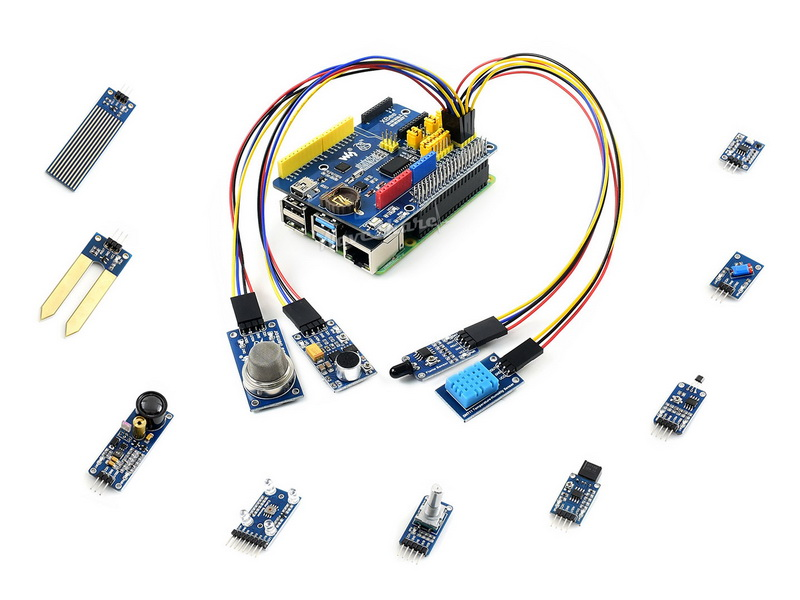
\includegraphics[keepaspectratio,width=\linewidth]{images/rpi-sens}
			\end{figure}
		\end{column}
	\end{columns}
\end{frame}

\begin{frame}{Fast, cheap, and secure IoT Defence -- pick 3?}
	\begin{columns}
		\begin{column}{0.4\linewidth}
			\begin{figure}
				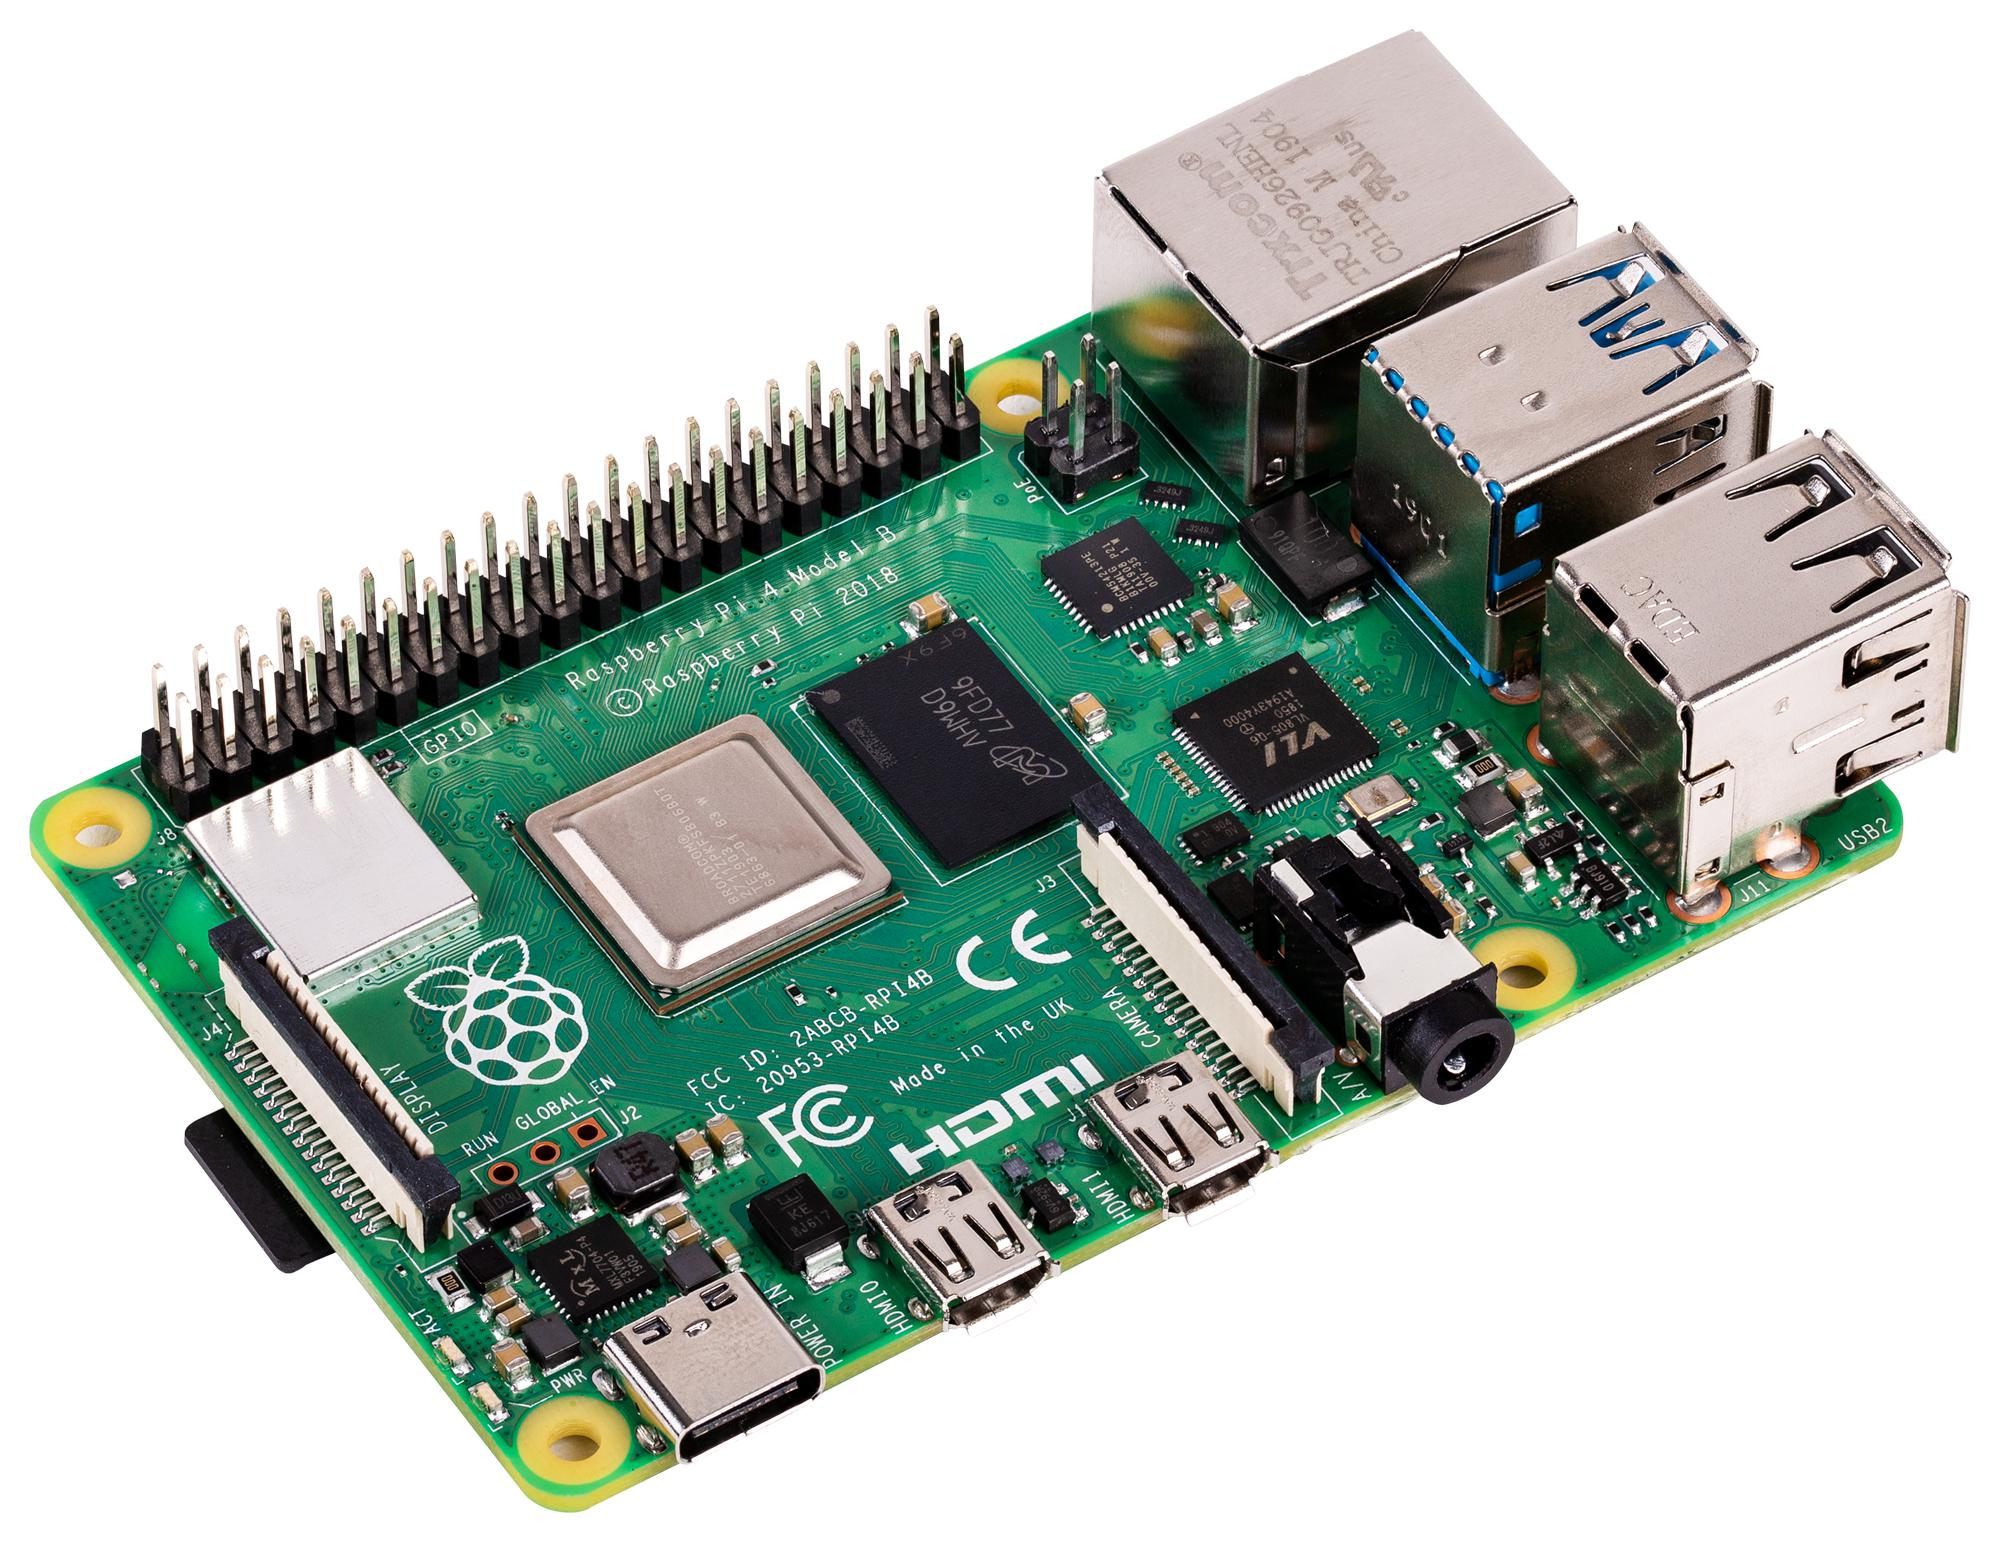
\includegraphics[keepaspectratio,width=\linewidth]{images/rpi}
			\end{figure}
		\end{column}
		\begin{column}{0.6\linewidth}
			%			\alert{A thing}: bright results!
			\begin{itemize}
				\item Single-board compute like RPis are small, capable, affordable! \alert{Cheap!}
				\begin{itemize}
					\item See also: NUCs (££), Jetsons (£££).
					\item \emph{Linux-based}: Easy(/ier) to target and write for. \alert{We also get kernel network stack advancements.}
					\item Different CPU architectures.
				\end{itemize}
				\item Sensor networks have low data rates; a good fit.
				\item Project goals:
				\begin{itemize}
					\item \alert{Fast!} Low-latency, quickly reconfigurable.
					\item \alert{Secure!} efficient NFV code gen from \emph{memory-safe languages}.
				\end{itemize}
			\end{itemize}
		\end{column}
	\end{columns}
\end{frame}

\begin{frame}{\ourtech{}'s Research Objectives}
	\begin{enumerate}
		\item What specialisations does XDP Function Chaining need to best suit SBCs?
		\begin{itemize}
			\item `Acceptably' low-latency packet-processing, without pushing CPU/power draw too high?
		\end{itemize}
		\item How do we make eBPF + native compile from memory-safe systems languages easy? And portable across `native'?
		\begin{itemize}
			\item One Rust program per NF $\implies$ compiles to eBPF + \mintinline{bash}|$PLATFORM|.
			\item Simple, dynamic chain format.
			\item Fast reconfiguration.
		\end{itemize}
		\item How much better is it [power, perf, lat]?
		\begin{itemize}
			\item With/without polling.
		\end{itemize}
	\end{enumerate}
%	\begin{itemize}
%%		\item ?? 3 things in my work now: how do we make joint compile in secure, memsafe lang easier? How do we specialize xdp sfc for cheaper devices? How much better is it [power, perf, lat]?
%		
%		\item Fast reconfiguration:
%		\begin{itemize}
%			\item State, Program Code, \alert{Composition}
%		\end{itemize}
%%		\item Attestation and authentication:
%%		\begin{itemize}
%%			\item Right programs on right machine, requested by trusted server.
%%		\end{itemize}
%		\item `Acceptably' low-latency packet-processing, without pushing CPU/power draw too high?
%		\begin{itemize}
%			\item I.e., as low as we can get without polling.
%		\end{itemize}
%		\item Easy development and composition.
%		\begin{itemize}
%			\item One Rust program per NF $\implies$ compiled for stack.
%			\item Simple, dynamic chain format.
%		\end{itemize}
%	\end{itemize}
\end{frame}

\section{Background}

\begin{frame}{Limits of existing SFC}
	\begin{itemize}
		\item `Best' low latency processing (DPDK) is \alert{expensive} -- CPU and power.
		\begin{itemize}
			\item ...IFF you have HW support (NUCs)
		\end{itemize}
%		\item SotA in \emph{secure} processing needs server-only capabilities like \emph{trusted execution environments} (TEEs).
		\item No powerful hardware offloads or acceleration.
		\begin{itemize}
			\item FPGA hats/daughterboards \alert{`off-path'}
		\end{itemize}
		\item Devices physically vulnerable, \alert{no ECC memory}.
		\item ...So, how to reconcile with cheap \& portable SBCs?
	\end{itemize}
\end{frame}

%\begin{frame}{What tools do we \emph{consistently} have?}
%	\begin{itemize}
%		\item SBCs often linux-based
%		\begin{itemize}
%			\item Easy(/ier) to target and write for.
%			\item \alert{Advantage:} We also get kernel network stack advancements.
%		\end{itemize}
%		\item Can run commodity software with no issues, reasonable target archs like Aarch64, x86\_64, ...
%		\item Includes, principally, eBPF tooling!
%%		\item XDP since 2016, \texttt{AF\_XDP} since 2019 (kver 4.18). more features in newer kernels! (recent: (\texttt{AF\_})XDP for windows)
%%		\item Key to XDP's value: stack bypass that \emph{improves} with driver support vs. builtin.
%	\end{itemize}
%\end{frame}

%\section{Hm?}

\begin{frame}{eBPF: What and Why?}
	\begin{columns}
		\begin{column}{0.6\linewidth}
			\begin{itemize}
				\item Simple register machine VM (user-written) code, derived from BPF.
				\item Modern use -- Kernel hooks, perf instrumentation, debugging
				\item JIT compiled
				\item Kernel-verified
				\begin{itemize}
					\item Bounds-checked pointer accesses
					\item Program size limited, no unbounded loops
					\item Syscalls (\emph{eBPF helpers}) exposed based on hook point
				\end{itemize}
			\end{itemize}
		\end{column}
		\begin{column}{0.4\linewidth}
			\begin{figure}
				\centering
				
\includegraphics[width=0.9\linewidth,keepaspectratio]{images/ebpf}
			\end{figure}
		\end{column}
	\end{columns}
\end{frame}

\begin{frame}{Network stack improvements: XDP}
	\begin{columns}
		\begin{column}{0.5\linewidth}
			\resizebox{\linewidth}{!}{
%				\colorlet{ol-phys}{uofgforest}
\colorlet{ol-log}{uofglavendar}
\colorlet{ol-user}{uofgrust}
\colorlet{ol-userland}{ol-user!75}

\colorlet{ol-arrow}{black}
\colorlet{ol-user-arrow}{ol-user}

\begin{tikzpicture}
	\draw[color=ol-phys,fill=ol-phys!10] (0,0) rectangle ++(2,1) node[pos=.5] (mac) {MAC};
	\draw[color=ol-phys,fill=ol-phys!10] ($(mac) + (2, -0.5)$) rectangle ++(2,1) node[pos=.5] (nic) {NIC};
	\draw[color=ol-phys,fill=ol-phys!10,align=center,text=black] ($(nic) + (2, -0.5)$) rectangle ++(2,1) node[pos=.5] (mem) {Memory\\\& Cache};

	\draw[color=ol-log,fill=ol-log!10,align=center,text=black] ($(mem) + (2, -0.5)$) rectangle ++(2,1) node[pos=.5] (rx-tx) {Driver\\Rx/Tx};
	\draw[color=ol-log,fill=ol-log!10,align=center,text=black] ($(rx-tx) + (-1, -2.5)$) rectangle ++(2,1) node[pos=.5] (skb) {Kernel\\SKB Alloc};
	\draw[color=ol-log,fill=ol-log!10,align=center,text=black] ($(skb) + (-1, -2.5)$) rectangle ++(2,1) node[pos=.5] (ns) {Network\\Stack};

	\draw[color=ol-userland, fill=ol-userland,align=center, text=white, rounded corners] ($(ns) + (-5, -0.5)$) rectangle ++(2,1) node[pos=.5] (userland) {Userland\\Code};

	\draw[color=ol-user, fill=ol-user,align=center,text=white, rounded corners] ($(nic) + (-2, -3.5)$) rectangle ++(2,1) node[pos=.5] (smartnic-offload) {Offload\\C/P4/eBPF};

	\draw[color=ol-user, fill=ol-user,align=center,text=white, rounded corners] ($(skb) + (-5, -0.5)$) rectangle ++(2,1) node[pos=.5] (xdp-offload) {Offload\\eBPF (XDP)};

	% --------

	\node[color=ol-phys] at (0.75, 1.35) {\large{}Physical};
	\node[color=ol-log, rotate=270] at (11.5, 0.5) {\large{}Logical};

	% --------

	\draw[<->, thick, color=ol-arrow] (mac) -- (nic);
	\draw[<->, thick, color=ol-arrow] (nic) -- (mem);
	\draw[<->, thick, color=ol-arrow] (mem) -- (rx-tx) node[midway, above] {\small{}IRQs};
	\draw[<->, thick, color=ol-arrow] (rx-tx) -- (skb);
	\draw[<->, thick, color=ol-arrow] (skb) -- (ns);


	\draw[<->, thick, color=ol-user-arrow, shorten >=0.25cm,shorten <=0.3cm] (ns) -- (userland) node[midway, below] {\small{}Socket};
	\draw[<->, thick, color=ol-user-arrow, shorten >=0.12cm,shorten <=0.17cm] (nic) -- (smartnic-offload) node[midway, left, align=center] {\small{}SmartNIC\\Offload};
	\draw[<->, thick, color=ol-user-arrow, shorten >=0.12cm,shorten <=0.12cm] (rx-tx) -- (xdp-offload) node[midway, above, sloped] {\small{}Native \color{ol-user-arrow}XDP};
	\draw[<->, thick, color=ol-user-arrow, shorten >=0.05cm,shorten <=0.12cm] (skb) -- (xdp-offload) node[midway, above] {\small{}Generic \color{ol-user-arrow}XDP};
	\draw[<->, thick, color=ol-user-arrow, shorten >=0.12cm,shorten <=0.12cm] (userland) -- (xdp-offload) node[midway, right] {\small{}\texttt{AF\_XDP}};

	\draw[<->, thick, color=ol-user-arrow, shorten >=0.12cm,shorten <=0.12cm, out=200,in=150] (mem) to node[left] {\small{}DPDK} (userland);
\end{tikzpicture}
\colorlet{ol-phys}{uofgforest}
\colorlet{ol-log}{uofglavendar}
\colorlet{ol-user}{uofgrust}
\colorlet{ol-userland}{ol-user!75}

\colorlet{ol-arrow}{black}
\colorlet{ol-user-arrow}{ol-user}

\begin{tikzpicture}
	\draw[color=ol-phys,fill=ol-phys!10] (0,0) rectangle ++(2,1) node[pos=.5] (mac) {MAC};
	\draw[color=ol-phys,fill=ol-phys!10] ($(mac) + (2, -0.5)$) rectangle ++(2,1) node[pos=.5] (nic) {NIC};
	\draw[color=ol-phys,fill=ol-phys!10,align=center,text=black] ($(nic) + (2, -0.5)$) rectangle ++(2,1) node[pos=.5] (mem) {Memory\\\& Cache};
	
	\draw[color=ol-log,fill=ol-log!10,align=center,text=black] ($(mem) + (2, -0.5)$) rectangle ++(2,1) node[pos=.5] (rx-tx) {Driver\\Rx/Tx};
	\draw[color=ol-log,fill=ol-log!10,align=center,text=black] ($(rx-tx) + (-1, -2.5)$) rectangle ++(2,1) node[pos=.5] (skb) {Kernel\\SKB Alloc};
	\draw[color=ol-log,fill=ol-log!10,align=center,text=black] ($(skb) + (-1, -2.5)$) rectangle ++(2,1) node[pos=.5] (ns) {Network\\Stack};
	
	\draw[color=ol-userland, fill=ol-userland,align=center, text=white, rounded corners] ($(ns) + (-5, -0.5)$) rectangle ++(2,1) node[pos=.5] (userland) {Userland\\Code};
	
	\draw[color=ol-user, fill=ol-user,align=center,text=white, rounded corners] ($(nic) + (-2, -3.5)$) rectangle ++(2,1) node[pos=.5] (smartnic-offload) {Offload\\C/P4/eBPF};
	
	\draw[color=ol-user, fill=ol-user,align=center,text=white, rounded corners] ($(skb) + (-5, -0.5)$) rectangle ++(2,1) node[pos=.5] (xdp-offload) {Offload\\eBPF (XDP)};
	
	% --------
	
	\node[color=ol-phys] at (0.75, 1.35) {\large{}Physical};
	\node[color=ol-log, rotate=270] at (11.5, 0.5) {\large{}Logical};
	
	% --------
	
	\draw[<->, thick, color=ol-arrow] (mac) -- (nic);
	\draw[<->, thick, color=ol-arrow] (nic) -- (mem);
	\draw[<->, thick, color=ol-arrow] (mem) -- (rx-tx) node[midway, above] {\small{}IRQs};
	\draw[<->, thick, color=ol-arrow] (rx-tx) -- (skb);
	\draw[<->, thick, color=ol-arrow] (skb) -- (ns);
	
	
	\draw[<->, thick, color=ol-user-arrow, shorten >=0.25cm,shorten <=0.3cm] (ns) -- (userland) node[midway, below] {\small{}Socket};
	\draw[<->, thick, color=ol-user-arrow, shorten >=0.12cm,shorten <=0.17cm] (nic) -- (smartnic-offload) node[midway, left, align=center] {\small{}SmartNIC\\Offload};
	\draw[<->, thick, color=ol-user-arrow, shorten >=0.12cm,shorten <=0.12cm] (rx-tx) -- (xdp-offload) node[midway, above, sloped] {\small{}Native \color{ol-user-arrow}XDP};
	\draw[<->, thick, color=ol-user-arrow, shorten >=0.05cm,shorten <=0.12cm] (skb) -- (xdp-offload) node[midway, above] {\small{}Generic \color{ol-user-arrow}XDP};
	\draw[<->, thick, color=ol-user-arrow, shorten >=0.12cm,shorten <=0.12cm] (userland) -- (xdp-offload) node[midway, right] {\small{}\texttt{AF\_XDP}};
	
	\draw[<->, thick, color=ol-user-arrow, shorten >=0.12cm,shorten <=0.12cm, out=200,in=150] (mem) to node[left] {\small{}DPDK} (userland);
\end{tikzpicture}
			}
		\end{column}
		\begin{column}{0.5\linewidth}
			\begin{itemize}
				\item eBPF hook attached to \alert{packet ingress}
				\item Variations on hook $\in \left\{\text{Offload, Driver, Generic}\right\}$
				\begin{itemize}
					\item Perf degrades gracefully according to driver support
				\end{itemize}
				\item Hook can modify \& inspect packets before forwarding to Linux stack, sending \alert{straight to (another) NIC}, or drop.
				\item Since 2019: \texttt{AF\_XDP} stack bypass!
			\end{itemize}
		\end{column}
	\end{columns}
\end{frame}

\section{Q1: Specialising \afxdp{} SFC to SBCs}

\begin{frame}{Concrete design differences}
	\begin{itemize}
		\item \textbf{Problem:} Mismatch of HW queues to physical cores:
		\begin{itemize}
			\item \alert{Soln:} load balance or place high-latency NFs in userland.
			\item ...also, don't pass packets back to k-space.
		\end{itemize}
		\item \textbf{Problem:} XDP hooks only on ingress (\emph{for now}):
		\begin{itemize}
			\item \alert{Soln:} load balance or place high-latency NFs in userland?
			\item Write an individual NF \emph{once}, compile for both envs, and replicate NFs as needed.
		\end{itemize}
	\end{itemize}
\end{frame}

\begin{frame}{Design: Bird's eye view}
	\begin{columns}
		\begin{column}{0.5\linewidth}
			\begin{figure}
				\centering
				\resizebox{0.9\linewidth}{!}{\hspace{-0.9cm}\tikzset{
	crate/.style n args={2}{%
		append after command={\pgfextra{\let\mainnode=\tikzlastnode}
			node[above] (cc) at (\mainnode.north) {
\includegraphics[keepaspectratio,width=1cm]{images/cargo}}%
			node at (cc.south) {#1}%
			node at (cc.west) {#2}%
		},
	}
}

\tikzset{
	file/.style n args={1}{%
		append after command={\pgfextra{\let\mainnode=\tikzlastnode}
			node[above] (cc) at (\mainnode.north) {\Huge\faFile*[regular]}%
			node[fill=white] at ($(cc.south) - (0,0.1)$) {\texttt{#1}}%
		},
	}
}

\tikzset{
	compile-both/.style n args={1}{%
		append after command={\pgfextra{\let\mainnode=\tikzlastnode}
			node[circle, draw, above left, fill=white] (cc) at (\mainnode) {\faMicrochip{}}%
			node[circle, draw, fill=white, inner sep=0pt,
			text width=7mm,align=center] at (\mainnode) {
\includegraphics[keepaspectratio,width=0.45cm]{images/ebpf}}%
			node[left] at (cc.west) {#1}%
		},
	}
}

\tikzset{
	compile/.style n args={1}{%
		append after command={\pgfextra{\let\mainnode=\tikzlastnode}
			node[circle, draw, above left, fill=white] (cc) at (\mainnode) {\faMicrochip{}}%
			node[left] at (cc.west) {#1}%
		},
	}
}

\tikzset{
	graphnode/.style={%
		fill=white,%
		circle,%
		draw,%
		text width=2mm,%
		align=center,%
		text=black%
	}
}

\tikzset{
	old inner xsep/.estore in=\oldinnerxsep,
	old inner ysep/.estore in=\oldinnerysep,
	double circle/.style 2 args={
		circle,
		old inner xsep=\pgfkeysvalueof{/pgf/inner xsep},
		old inner ysep=\pgfkeysvalueof{/pgf/inner ysep},
		/pgf/inner xsep=\oldinnerxsep+#1,
		/pgf/inner ysep=\oldinnerysep+#1,
		alias=sourcenode,
		append after command={
			let     \p1 = (sourcenode.center),
			\p2 = (sourcenode.east),
			\n1 = {\x2-\x1-#1-0.5*\pgflinewidth}
			in
			node [inner sep=0pt, draw, circle, minimum width=2*\n1,at=(\p1),#2] {}
		}
	},
	double circle/.default={2pt}{blue}
}

\tikzset{
	graphnode-terminal/.style n args={1}{%
		fill={#1},%
		double circle={-2pt}{#1},%
		circle,%
		draw,%
%		text width=2mm,%
		align=center,%
		text=white%
	},
	graphnode-terminal/.default={black}
}

\tikzset{
	nicebox/.style={draw,rounded corners,color=uofgsandstone,fill=uofgsandstone!10,dashed},
	gpath/.style={color=uofgheather,thick},
	usepath/.style={color=uofgmocha,thick},
	daemonbox/.style={draw, rounded corners, fill=white,align=center,},
	authbox/.style={draw, rounded corners, fill=uofgpumpkin!30, align=center,},
	client-authbox/.style={authbox,minimum width=1.8cm,rotate=90},
	authflow/.style={color=uofgthistle,thick},
	normflow/.style={color=uofgpillarbox,thick,dash dot},
}

\tikzset{
	map-cyl/.style n args={1}{%
		cylinder, shape border rotate=90, draw,align=center,aspect=0.1,font={\small},%
		cylinder uses custom fill, cylinder end fill=#1!50, cylinder body fill = #1!10
	},
	map-cyl/.default={uofgsandstone}
}

\begin{tikzpicture}
	\draw[nicebox] (0.45,-1.45) rectangle ++(3.5,2.9);
	\draw[nicebox] (-3.85,-1.4) rectangle ++(3.2,2.75);
	\node (compiler-infra) {
		\begin{tikzpicture}
			\node[crate={ACL} {a)}] (acl-crate) {};
			\node[crate={Rate Check} {b)}] at (1.5,0) (rate-crate) {};
%			\node[crate={\faLock{} DPI} {c)}] at (0, -1.5) (dpi-crate) {};
			\node[crate={DPI} {c)}] at (0, -1.5) (dpi-crate) {};
			\node[crate={Stats} {d)}] at (1.5,-1.5) (stats-crate) {};
			
			\node[draw, rounded corners, rotate=90] at (2.9,-0.25) (compiler) {\texttt{rustc} \& RedBPF};
			
			\draw[->,normflow] ($(compiler.north west) - (0.3,-0.3)$) -- ($(compiler.north west) - (0,-0.3)$);
			\draw[->,normflow] ($(compiler.north east) - (0.3,0.3)$) -- ($(compiler.north east) - (0,0.3)$);
			\draw[->,normflow] ($(compiler.south west) - (0,-0.3)$) -- ($(compiler.south west) + (0.3,0.3)$);
			\draw[->,normflow] ($(compiler.south east) - (0,0.3)$) -- ($(compiler.south east) + (0.3,-0.3)$);
			
			\node[compile-both={a)}] (acl-comp) at ($(acl-crate) + (4.75,0.4)$) {};
			\node[compile-both={b)}] (rate-comp) at ($(acl-comp) + (1.75,0)$) {};
			\node[compile={c)}] (dpi-comp) at ($(acl-comp) + (0,-1.5)$) {};
			\node[compile-both={d)}] (stats-comp) at ($(dpi-comp) + (1.75,0)$) {};
		\end{tikzpicture}
	};

	\node (chain) at ($(compiler-infra) + (-0.68, -2.7)$) {
		\begin{tikzpicture}
			\node[nicebox] (chainbox) {
				\begin{tikzpicture}
					\node[graphnode-terminal=uofgheather] (rx) {\textsc{Rx}};
					\node[graphnode] (a-node) at ($(rx) + (0,-1)$) {a};
					\node[graphnode] (b-node) at ($(a-node) + (1,0)$) {b};
					\node[graphnode] (c-node) at ($(b-node) + (1,0)$) {c};
					\node[graphnode] (d-node) at ($(b-node) + (0.5,1)$) {d};
					
					\node[graphnode-terminal=uofgpillarbox] (drop) at ($(b-node) + (2,0)$) {\tiny\textsc{Drop}};
					\node[graphnode-terminal=uofgcobalt] (tx) at ($(d-node) + (1,0)$) {\textsc{Tx}};
					
					\draw[->, gpath] (rx) -- (a-node);
					
					\draw[->, gpath] (a-node) -- (b-node);
					\draw[->, gpath] (a-node) to[out=-30, in=210] (drop);
					
					\draw[->, gpath] (b-node) -- (c-node);
					\draw[->, gpath] (b-node) -- (d-node);
					
					\draw[->, gpath] (c-node) -- (d-node);
					\draw[->, gpath] (c-node) -- (drop);
					
					\draw[->, gpath] (d-node) -- (tx);
				\end{tikzpicture}
			};
		
		\node[file={chain.toml}] (toml) at (3.5,-0.5) {};
		
		\draw[dotted, color=uofgsandstone] (chainbox.north east) -- ($(toml.west) + (-0.2,1.1)$);
		\draw[dotted, color=uofgsandstone] (chainbox.south east) -- ($(toml.west) + (-0.2,0.2)$);
		\end{tikzpicture}
	};
	
	% ------------------
	
%	\node (xdp-chain) at ($(daemon-client) + (4, -1.4)$) {
	\node (xdp-chain) at (0, -8) {\resizebox{7cm}{!}{
		\begin{tikzpicture}
			\draw[draw=black, fill=white, rounded corners] (0.3,0.3) rectangle ++(3,0.8);
			\draw[draw=black, fill=white, rounded corners] (0.15,0.15) rectangle ++(3,0.8);
			\draw[draw=black, fill=white, rounded corners] (0,0) rectangle ++(3,0.8);
			
			\node[graphnode] (c-node') at (0.5,0.4) {c};
			\node[graphnode] (d-node') at ($(c-node') + (1,0)$) {d};
			\node[graphnode-terminal=uofgpillarbox] (drop') at ($(d-node') + (1,0)$) {D};
			
			\node[graphnode] (a-node) at (0.15,-2) {a};
			\node[graphnode] (b-node) at ($(a-node) + (1,0)$) {b};
			\node[graphnode] (d-node) at ($(b-node) + (1,0)$) {d};
			
			\node[graphnode-terminal=uofgheather] (rx) at (0,-3.5) {\textsc{Rx}};
			\node[graphnode-terminal=uofgpillarbox] (drop) at ($(rx) + (1.5,0)$) {D};
			\node[graphnode-terminal=uofgcobalt] (tx) at ($(rx) + (3,0)$) {\textsc{Tx}};
			
			\node (hwt) at ($(tx) + (1,0)$) {\textsc{Hw}};
			\node[align=center] (xdpt) at ($(d-node) + (2.15,0)$) {\textsc{XDP Fast}\\\textsc{Path} 
\includegraphics[keepaspectratio,width=1em]{images/ebpf}};
			\node[align=center] (usrt) at ($(drop') + (1.8,0)$) {\textsc{User} \faMicrochip \\(\textsc{AArch64})};
			
			\draw[dashed, color=uofgsandstone] (-0.5,-1) -- (4.25,-1);
			\draw[dashed, color=uofgsandstone] (-0.5,-2.75) -- (4.25,-2.75);
			
%			\draw[dashed, color=uofgsandstone] (-0.5,-2.75) -- (-0.5,1);
%			\draw[dashed, color=uofgsandstone] (-2.25,-2.75) -- (-2.25,-3.9);
			
			\node[draw,fill=uofgsandstone!10,rounded corners,align=center] (maps) at (1.5,-1) {BPF Maps\\(State)};
			
			\draw[->, gpath] (rx) -- (a-node);
			
			\draw[->, gpath] (a-node) -- (b-node);
			\draw[->, gpath] (a-node) -- (drop);
			
			\draw[->, gpath, dashed] (b-node) to[in=-120, out=150] (c-node');
			\draw[->, gpath] (b-node) -- (d-node);
			
			\draw[->, gpath] (c-node') -- (d-node');
			\draw[->, gpath] (c-node') to[in=150, out=30] (drop');
			
			\draw[->, gpath] (d-node) -- (tx);
			\draw[->, gpath, dashed] (d-node') to[out=-30, in=90] (tx);
			
			\node[gpath, font={\small}] at ($(b-node) + (-1.55,0.5)$) {\texttt{AF\_XDP}};
			\node[gpath, font={\small}] at ($(drop') + (0.8,-1)$) {\texttt{AF\_XDP}};
			
			\draw[->, usepath] ($(maps.north) + (0, 0.4)$) -- ($(maps.north)$);
			\draw[->, usepath] ($(maps.north) + (-0.5, 0.2)$) -- ($(maps.north) - (0.2,0)$);
			\draw[->, usepath] ($(maps.north) + (0.5, 0.2)$) -- ($(maps.north) + (0.2,0)$);
			
			\draw[->, usepath] ($(maps.south) + (0, -0.4)$) -- ($(maps.south)$);
			\draw[->, usepath] ($(maps.south) + (-0.5, -0.2)$) -- ($(maps.south) - (0.2,0)$);
			\draw[->, usepath] ($(maps.south) + (0.5, -0.2)$) -- ($(maps.south) + (0.2,0)$);
		\end{tikzpicture}
	}
	};
	
	% --- dividing lines
	\draw[color=uofgsandstone!50, dashed, thick] (-5,-4.5) -- (5,-4.5);
	\node[align=center] (tee) at (4,-4.3) {\textsc{Remote Compile Server}};
	\node[align=center] (tee) at (4,-5.1) {\textsc{SBC Traffic}\\\textsc{Processor}};
	
	% --- NF flow
	\draw[->, normflow] ([yshift=0.0cm]compiler-infra.south east) to[out=-20,in=45] node[midway, below, xshift=0.8cm,yshift=0.0cm] {NF Binaries} (xdp-chain.north);
	\draw[->, normflow] (chain.south) to[out=-20,in=90] node[pos=0.3, below,yshift=-0.3cm,xshift=-1cm] {NF Config} ([xshift=-0.3cm]xdp-chain.north);
%	\draw[<->, normflow] (daemon-server.north) to[out=20,in=160] node[midway, above, fill=white,yshift=0.1cm] {NFs, Queries, Stats} (daemon-client.north);
\end{tikzpicture}\hspace{-0.2cm}}
			\end{figure}
		\end{column}
		\begin{column}{0.5\linewidth}
			\begin{itemize}
				\item Two-tier approach---XDP \& User.
				\item Composable NFs -- graph structure.
				\item Critical or high performance NFs go into XDP:
				\begin{itemize}
					\item Early results -- \alert{low latency for most packets}.
				\end{itemize}
				\item Rare `slow-path' still kernel bypass:
				\begin{itemize}
					\item Expensive \& proprietary code.
					\item Only for candidate attack traffic.
				\end{itemize}
				\item Reconfigurable, dynamic.
			\end{itemize}
		\end{column}
	\end{columns}
\end{frame}

\begin{frame}{How does this differ from other frameworks?}
	\textbf{In Security?} SafeBricks~\footcite{DBLP:conf/nsdi/PoddarLPR18}, AuditBox~\footcite{DBLP:conf/nsdi/LiuSKPSS21} or similar.
	\begin{itemize}
		\item ...No SGX support in devices of interest.
	\end{itemize}
	
	\textbf{In eBPF/XDP space?} Polycube~\footcite{DBLP:journals/tnsm/MianoRBBL21}!
	\begin{itemize}
		\item Built around datacentres -- we often have just one HW queue for a NIC.
	\end{itemize}
\end{frame}

\begin{frame}{How do we upcall to userland?}
	\begin{itemize}
		\item \textbf{Problem:} Can send packet over \texttt{AF\_XDP}, but \emph{no context on what the next (callee) NF is}.
		\begin{itemize}
			\item Polycube's solution inadequate: one discrete userland component per \emph{cube}.
		\end{itemize}
		\item \alert{Soln:} Adjust headroom of packets, write in ID and action of caller.
		\item ...might be a \texttt{memcpy}, but ideally only paid on packets who need it.
	\end{itemize}
\end{frame}

\section{Q2: Easy Joint-Compile (eBPF + Native) from Rust \twemoji{crab}}

\begin{frame}[fragile=singleslide]{Skeleton details}
	\begin{columns}
		\begin{column}{0.5\linewidth}
			\begin{itemize}
				%				\item ?? Discuss API etc here in more detail?
				\item Consistent NF API for both XDP/userland.
				\item Rust compiler should be able to enforce...
				\begin{itemize}
					\item \mintinline{rust}|#![forbid(unsafe_code)]| (or similar cargo tooling) on NF module crates,
					\item all NF branches specified.
				\end{itemize}
				\item All compilation on external server.
				\begin{itemize}
					\item SBC too constrained.
					\item If compile-server is TEE-equipped, \alert{can attest compiler/code} etc. following SotA!
				\end{itemize}
			\end{itemize}
		\end{column}
		\begin{column}{0.5\linewidth}
			\centering
			\begin{minted}[fontsize={\fontsize{5.5}{6.5}\selectfont}]{rust}
#![no_std]
pub enum Action {
	Left,
	Right,
	Up,
	Down,
}
				
pub fn packet(bytes: impl Packet) -> Action {
	let addr_lsb_idx = 14 +
	match pkt.slice_from(12, 2) {
		Some(&[0x08, 0x00]) => 19, //v4
		Some(&[0x86, 0xDD]) => 39, //v6
		_ => {return Action::Left},
	};
	
	match pkt.slice_from(addr_lsb_idx, 1)
		.map(|v| v[0] % 2) {
			Some(0) => Action::Left,
			Some(1) => Action::Right,
			Some(2) => Action::Up,
			Some(3) => Action::Down,
			_ => unreachable!(),
	}
}
			\end{minted}
			\textbf{\texttt{mod.rs}: Load balance on dest addr}
		\end{column}
	\end{columns}
\end{frame}

\begin{frame}{?? Chain example}
	\centering
	\textbf{\alert{< In lieu of a demo... >}}
\end{frame}

%\begin{frame}{Methodology (I): Low-latency XDP fast-path}
%	\begin{columns}
%		\begin{column}{0.5\linewidth}
%			\begin{figure}
%				\centering
%				\resizebox{0.9\linewidth}{!}{\hspace{-0.9cm}\tikzset{
	crate/.style n args={2}{%
		append after command={\pgfextra{\let\mainnode=\tikzlastnode}
			node[above] (cc) at (\mainnode.north) {
\includegraphics[keepaspectratio,width=1cm]{images/cargo}}%
			node at (cc.south) {#1}%
			node at (cc.west) {#2}%
		},
	}
}

\tikzset{
	file/.style n args={1}{%
		append after command={\pgfextra{\let\mainnode=\tikzlastnode}
			node[above] (cc) at (\mainnode.north) {\Huge\faFile*[regular]}%
			node[fill=white] at ($(cc.south) - (0,0.1)$) {\texttt{#1}}%
		},
	}
}

\tikzset{
	compile-both/.style n args={1}{%
		append after command={\pgfextra{\let\mainnode=\tikzlastnode}
			node[circle, draw, above left, fill=white] (cc) at (\mainnode) {\faMicrochip{}}%
			node[circle, draw, fill=white, inner sep=0pt,
			text width=7mm,align=center] at (\mainnode) {
\includegraphics[keepaspectratio,width=0.45cm]{images/ebpf}}%
			node[left] at (cc.west) {#1}%
		},
	}
}

\tikzset{
	compile/.style n args={1}{%
		append after command={\pgfextra{\let\mainnode=\tikzlastnode}
			node[circle, draw, above left, fill=white] (cc) at (\mainnode) {\faMicrochip{}}%
			node[left] at (cc.west) {#1}%
		},
	}
}

\tikzset{
	graphnode/.style={%
		fill=white,%
		circle,%
		draw,%
		text width=2mm,%
		align=center,%
		text=black%
	}
}

\tikzset{
	old inner xsep/.estore in=\oldinnerxsep,
	old inner ysep/.estore in=\oldinnerysep,
	double circle/.style 2 args={
		circle,
		old inner xsep=\pgfkeysvalueof{/pgf/inner xsep},
		old inner ysep=\pgfkeysvalueof{/pgf/inner ysep},
		/pgf/inner xsep=\oldinnerxsep+#1,
		/pgf/inner ysep=\oldinnerysep+#1,
		alias=sourcenode,
		append after command={
			let     \p1 = (sourcenode.center),
			\p2 = (sourcenode.east),
			\n1 = {\x2-\x1-#1-0.5*\pgflinewidth}
			in
			node [inner sep=0pt, draw, circle, minimum width=2*\n1,at=(\p1),#2] {}
		}
	},
	double circle/.default={2pt}{blue}
}

\tikzset{
	graphnode-terminal/.style n args={1}{%
		fill={#1},%
		double circle={-2pt}{#1},%
		circle,%
		draw,%
%		text width=2mm,%
		align=center,%
		text=white%
	},
	graphnode-terminal/.default={black}
}

\tikzset{
	nicebox/.style={draw,rounded corners,color=uofgsandstone,fill=uofgsandstone!10,dashed},
	gpath/.style={color=uofgheather,thick},
	usepath/.style={color=uofgmocha,thick},
	daemonbox/.style={draw, rounded corners, fill=white,align=center,},
	authbox/.style={draw, rounded corners, fill=uofgpumpkin!30, align=center,},
	client-authbox/.style={authbox,minimum width=1.8cm,rotate=90},
	authflow/.style={color=uofgthistle,thick},
	normflow/.style={color=uofgpillarbox,thick,dash dot},
}

\tikzset{
	map-cyl/.style n args={1}{%
		cylinder, shape border rotate=90, draw,align=center,aspect=0.1,font={\small},%
		cylinder uses custom fill, cylinder end fill=#1!50, cylinder body fill = #1!10
	},
	map-cyl/.default={uofgsandstone}
}

\begin{tikzpicture}
	\draw[nicebox] (0.45,-1.45) rectangle ++(3.5,2.9);
	\draw[nicebox] (-3.85,-1.4) rectangle ++(3.2,2.75);
	\node (compiler-infra) {
		\begin{tikzpicture}
			\node[crate={ACL} {a)}] (acl-crate) {};
			\node[crate={Rate Check} {b)}] at (1.5,0) (rate-crate) {};
%			\node[crate={\faLock{} DPI} {c)}] at (0, -1.5) (dpi-crate) {};
			\node[crate={DPI} {c)}] at (0, -1.5) (dpi-crate) {};
			\node[crate={Stats} {d)}] at (1.5,-1.5) (stats-crate) {};
			
			\node[draw, rounded corners, rotate=90] at (2.9,-0.25) (compiler) {\texttt{rustc} \& RedBPF};
			
			\draw[->,normflow] ($(compiler.north west) - (0.3,-0.3)$) -- ($(compiler.north west) - (0,-0.3)$);
			\draw[->,normflow] ($(compiler.north east) - (0.3,0.3)$) -- ($(compiler.north east) - (0,0.3)$);
			\draw[->,normflow] ($(compiler.south west) - (0,-0.3)$) -- ($(compiler.south west) + (0.3,0.3)$);
			\draw[->,normflow] ($(compiler.south east) - (0,0.3)$) -- ($(compiler.south east) + (0.3,-0.3)$);
			
			\node[compile-both={a)}] (acl-comp) at ($(acl-crate) + (4.75,0.4)$) {};
			\node[compile-both={b)}] (rate-comp) at ($(acl-comp) + (1.75,0)$) {};
			\node[compile={c)}] (dpi-comp) at ($(acl-comp) + (0,-1.5)$) {};
			\node[compile-both={d)}] (stats-comp) at ($(dpi-comp) + (1.75,0)$) {};
		\end{tikzpicture}
	};

	\node (chain) at ($(compiler-infra) + (-0.68, -2.7)$) {
		\begin{tikzpicture}
			\node[nicebox] (chainbox) {
				\begin{tikzpicture}
					\node[graphnode-terminal=uofgheather] (rx) {\textsc{Rx}};
					\node[graphnode] (a-node) at ($(rx) + (0,-1)$) {a};
					\node[graphnode] (b-node) at ($(a-node) + (1,0)$) {b};
					\node[graphnode] (c-node) at ($(b-node) + (1,0)$) {c};
					\node[graphnode] (d-node) at ($(b-node) + (0.5,1)$) {d};
					
					\node[graphnode-terminal=uofgpillarbox] (drop) at ($(b-node) + (2,0)$) {\tiny\textsc{Drop}};
					\node[graphnode-terminal=uofgcobalt] (tx) at ($(d-node) + (1,0)$) {\textsc{Tx}};
					
					\draw[->, gpath] (rx) -- (a-node);
					
					\draw[->, gpath] (a-node) -- (b-node);
					\draw[->, gpath] (a-node) to[out=-30, in=210] (drop);
					
					\draw[->, gpath] (b-node) -- (c-node);
					\draw[->, gpath] (b-node) -- (d-node);
					
					\draw[->, gpath] (c-node) -- (d-node);
					\draw[->, gpath] (c-node) -- (drop);
					
					\draw[->, gpath] (d-node) -- (tx);
				\end{tikzpicture}
			};
		
		\node[file={chain.toml}] (toml) at (3.5,-0.5) {};
		
		\draw[dotted, color=uofgsandstone] (chainbox.north east) -- ($(toml.west) + (-0.2,1.1)$);
		\draw[dotted, color=uofgsandstone] (chainbox.south east) -- ($(toml.west) + (-0.2,0.2)$);
		\end{tikzpicture}
	};
	
	% ------------------
	
%	\node (xdp-chain) at ($(daemon-client) + (4, -1.4)$) {
	\node (xdp-chain) at (0, -8) {\resizebox{7cm}{!}{
		\begin{tikzpicture}
			\draw[draw=black, fill=white, rounded corners] (0.3,0.3) rectangle ++(3,0.8);
			\draw[draw=black, fill=white, rounded corners] (0.15,0.15) rectangle ++(3,0.8);
			\draw[draw=black, fill=white, rounded corners] (0,0) rectangle ++(3,0.8);
			
			\node[graphnode] (c-node') at (0.5,0.4) {c};
			\node[graphnode] (d-node') at ($(c-node') + (1,0)$) {d};
			\node[graphnode-terminal=uofgpillarbox] (drop') at ($(d-node') + (1,0)$) {D};
			
			\node[graphnode] (a-node) at (0.15,-2) {a};
			\node[graphnode] (b-node) at ($(a-node) + (1,0)$) {b};
			\node[graphnode] (d-node) at ($(b-node) + (1,0)$) {d};
			
			\node[graphnode-terminal=uofgheather] (rx) at (0,-3.5) {\textsc{Rx}};
			\node[graphnode-terminal=uofgpillarbox] (drop) at ($(rx) + (1.5,0)$) {D};
			\node[graphnode-terminal=uofgcobalt] (tx) at ($(rx) + (3,0)$) {\textsc{Tx}};
			
			\node (hwt) at ($(tx) + (1,0)$) {\textsc{Hw}};
			\node[align=center] (xdpt) at ($(d-node) + (2.15,0)$) {\textsc{XDP Fast}\\\textsc{Path} 
\includegraphics[keepaspectratio,width=1em]{images/ebpf}};
			\node[align=center] (usrt) at ($(drop') + (1.8,0)$) {\textsc{User} \faMicrochip \\(\textsc{AArch64})};
			
			\draw[dashed, color=uofgsandstone] (-0.5,-1) -- (4.25,-1);
			\draw[dashed, color=uofgsandstone] (-0.5,-2.75) -- (4.25,-2.75);
			
%			\draw[dashed, color=uofgsandstone] (-0.5,-2.75) -- (-0.5,1);
%			\draw[dashed, color=uofgsandstone] (-2.25,-2.75) -- (-2.25,-3.9);
			
			\node[draw,fill=uofgsandstone!10,rounded corners,align=center] (maps) at (1.5,-1) {BPF Maps\\(State)};
			
			\draw[->, gpath] (rx) -- (a-node);
			
			\draw[->, gpath] (a-node) -- (b-node);
			\draw[->, gpath] (a-node) -- (drop);
			
			\draw[->, gpath, dashed] (b-node) to[in=-120, out=150] (c-node');
			\draw[->, gpath] (b-node) -- (d-node);
			
			\draw[->, gpath] (c-node') -- (d-node');
			\draw[->, gpath] (c-node') to[in=150, out=30] (drop');
			
			\draw[->, gpath] (d-node) -- (tx);
			\draw[->, gpath, dashed] (d-node') to[out=-30, in=90] (tx);
			
			\node[gpath, font={\small}] at ($(b-node) + (-1.55,0.5)$) {\texttt{AF\_XDP}};
			\node[gpath, font={\small}] at ($(drop') + (0.8,-1)$) {\texttt{AF\_XDP}};
			
			\draw[->, usepath] ($(maps.north) + (0, 0.4)$) -- ($(maps.north)$);
			\draw[->, usepath] ($(maps.north) + (-0.5, 0.2)$) -- ($(maps.north) - (0.2,0)$);
			\draw[->, usepath] ($(maps.north) + (0.5, 0.2)$) -- ($(maps.north) + (0.2,0)$);
			
			\draw[->, usepath] ($(maps.south) + (0, -0.4)$) -- ($(maps.south)$);
			\draw[->, usepath] ($(maps.south) + (-0.5, -0.2)$) -- ($(maps.south) - (0.2,0)$);
			\draw[->, usepath] ($(maps.south) + (0.5, -0.2)$) -- ($(maps.south) + (0.2,0)$);
		\end{tikzpicture}
	}
	};
	
	% --- dividing lines
	\draw[color=uofgsandstone!50, dashed, thick] (-5,-4.5) -- (5,-4.5);
	\node[align=center] (tee) at (4,-4.3) {\textsc{Remote Compile Server}};
	\node[align=center] (tee) at (4,-5.1) {\textsc{SBC Traffic}\\\textsc{Processor}};
	
	% --- NF flow
	\draw[->, normflow] ([yshift=0.0cm]compiler-infra.south east) to[out=-20,in=45] node[midway, below, xshift=0.8cm,yshift=0.0cm] {NF Binaries} (xdp-chain.north);
	\draw[->, normflow] (chain.south) to[out=-20,in=90] node[pos=0.3, below,yshift=-0.3cm,xshift=-1cm] {NF Config} ([xshift=-0.3cm]xdp-chain.north);
%	\draw[<->, normflow] (daemon-server.north) to[out=20,in=160] node[midway, above, fill=white,yshift=0.1cm] {NFs, Queries, Stats} (daemon-client.north);
\end{tikzpicture}\hspace{-0.2cm}}
%			\end{figure}
%		\end{column}
%		\begin{column}{0.5\linewidth}
%			\begin{itemize}
%				\item Two-tier approach---XDP \& User.
%				\item Composable NFs -- graph structure.
%				\item Critical or high performance NFs go into XDP:
%				\begin{itemize}
%					\item Early results -- \alert{low latency for most packets}.
%				\end{itemize}
%				\item Rare `slow-path' still kernel bypass:
%				\begin{itemize}
%					\item Expensive \& proprietary code.
%					\item Only for candidate attack traffic.
%				\end{itemize}
%				\item Reconfigurable, dynamic.
%			\end{itemize}
%		\end{column}
%	\end{columns}
%\end{frame}

%\begin{frame}{Control plane: PUF-based authentication}
%	\begin{itemize}
%		\item How to attest the above code and config is correct?
%		\begin{itemize}
%			\item TLS w/ pre-shared certs works well.
%			\item But \alert{corruption, unplanned expiry possible on field devices}.
%		\end{itemize}
%		\item \alert{\emph{Physical Unclonable Functions} (PUFs)} -- input-based device signatures, CRPs.
%		\item Authenticate keys in the wild without root certs.
%		\begin{itemize}
%			\item Two-way: Client $\leftrightarrow$ Server!
%			\item Soln: RusTLS modification to declare challenge via X.509 extension, mix response bits into signature algo input [Zero-knowledge].
%		\end{itemize}
%		\item Strong attestation of identities to physical devices.
%	\end{itemize}
%\end{frame}
%
%\begin{frame}{Control plane: PUF-based authentication (II)}
%	\begin{columns}
%		\begin{column}{0.5\linewidth}
%			\begin{itemize}
%				\item \alert{RTD}-based array designs -- quantum property.
%				\item Behaviour in purple region (NDR region) \alert{physical device-dependent}
%				\begin{itemize}
%					\item Perturbations from `ideal' behaviour can't be replicated
%					\item N\unit{\degree} peaks and perturbations depend on active devices.
%				\end{itemize}
%				\item Challenge bits control used transistors in circuit
%				\begin{itemize}
%					\item $\sim$ Exp amount in $n$, Large Resp.
%				\end{itemize}
%			\end{itemize}
%		\end{column}
%		\begin{column}{0.5\linewidth}
%			\begin{figure}
%				\centering
%				\resizebox{\linewidth}{!}{\hspace{-1cm}\colorlet{challengecolour}{uofgcobalt}
\colorlet{challengemapcolour}{challengecolour!40}

\colorlet{respcolour}{uofgthistle}

\begin{tikzpicture}
	\node (circuit) at (0,0) {\resizebox{4cm}{!}{
		\begin{circuitikz}
%			\draw (0,0) to[short, o-*] (1,0) to [cuteopenswitchshape] (2,0) to[tDo] (3,0);
			
			% main block
			
			\node [cuteopenswitchshape] (sw1) at (2,2) {};
			\draw (sw1.out) to[tDo] ++(1,0) to[short, -*] ++(1,0) -- ++(0,-3);
			
			\node [cuteclosedswitchshape] (sw2) at ($(sw1) - (0,1)$) {};
			\draw (sw2.out) to[tDo] ++(1,0) to[short, -*] ++(1,0);
			
			\node [cuteclosedswitchshape] (sw3) at ($(sw2) - (0,1)$) {};
			\draw (sw3.out) to[tDo] ++(1,0) to[short, -*] ++(1,0);
			
			\node [cuteopenswitchshape] (sw4) at ($(sw3) - (0,1)$) {};
			\draw (sw4.out) to[tDo] ++(1,0) to[short, -*] ++(1,0);
			
			% routing to main block
			\draw (sw1.in) -- ++(-1, 0) -- ++(0,-3) -- ++(1,0);
			\draw (sw2.in) to[short,-*] ++(-1, 0);
			\draw (sw3.in) to[short,-*] ++(-1, 0);
			
			% dashed block
			
			\draw ($(sw1.out) + (2,0)$) -- ++(0.5,0);
			\draw[dashed] ($(sw1.out) + (2.5,0)$) -- ++(1,0);
			\draw ($(sw1.out) + (3.5,0)$) -- ++(0.5,0);
			
			\draw ($(sw2.out) + (2,0)$) -- ++(0.5,0);
			\draw[dashed] ($(sw2.out) + (2.5,0)$) -- ++(1,0);
			\draw ($(sw2.out) + (3.5,0)$) to[short, -*] ++(0.5,0);
			
			\draw ($(sw3.out) + (2,0)$) -- ++(0.5,0);
			\draw[dashed] ($(sw3.out) + (2.5,0)$) -- ++(1,0);
			\draw ($(sw3.out) + (3.5,0)$) to[short, -*] ++(0.5,0);
			
			\draw ($(sw4.out) + (2,0)$) -- ++(0.5,0);
			\draw[dashed] ($(sw4.out) + (2.5,0)$) -- ++(1,0);
			\draw ($(sw4.out) + (3.5,0)$) -- ++(0.5,0) -- ++(0,3);
			
			%output
			\draw ($(sw3.out) + (4,0.5)$) to[short,*-] ++(1,0);
			
			%input
			\draw ($(sw3.in) + (-1,0.5)$) to[short,*-] ++(-1,0);
			
		\end{circuitikz}
	}};

	% Challenge
	\node[text=challengecolour,font=\scriptsize] (cval) at ($(circuit) + (0,1.3)$) {\texttt{0110\hspace{0.15em}1101\hspace{0.15em}....}};
	\node[text=challengecolour,font=\scriptsize] (ctext) at ($(cval) + (-0.2,0.25)$) {Challenge: $n$ bits};
	
	\node (boxstart) at ($(cval) - (1.1,-0.2)$) {};
	\draw[color=challengecolour, thick] (boxstart) -- ++(0,-0.4) -- ++ (2.2,0) -- ++ (0, 0.28);
	\draw[color=challengecolour, thick] ($(boxstart) + (0.75,-0.4)$) -- ++(0,0.1);
	\draw[color=challengecolour, thick] ($(boxstart) + (1.45,-0.4)$) -- ++(0,0.1);
	
	% Challenge map
	\draw[color=challengemapcolour, densely dotted, thick] ($(boxstart) + (0,-0.4)$) -- ++(-0.33,-0.4);
	\draw[color=challengemapcolour, densely dotted, thick] ($(boxstart) + (0.75,-0.4)$) -- ++(0.8,-0.4);
	\draw[color=challengemapcolour!50, densely dotted, thick] ($(boxstart) + (1.45,-0.4)$) -- ++(0.3,-0.2);
	\draw[color=challengemapcolour, densely dotted, thick] ($(boxstart) + (2.2,-0.4)$) -- ++(0.35,-0.4);
	
	% Resp graph
%	\node (rg) at (3,1) {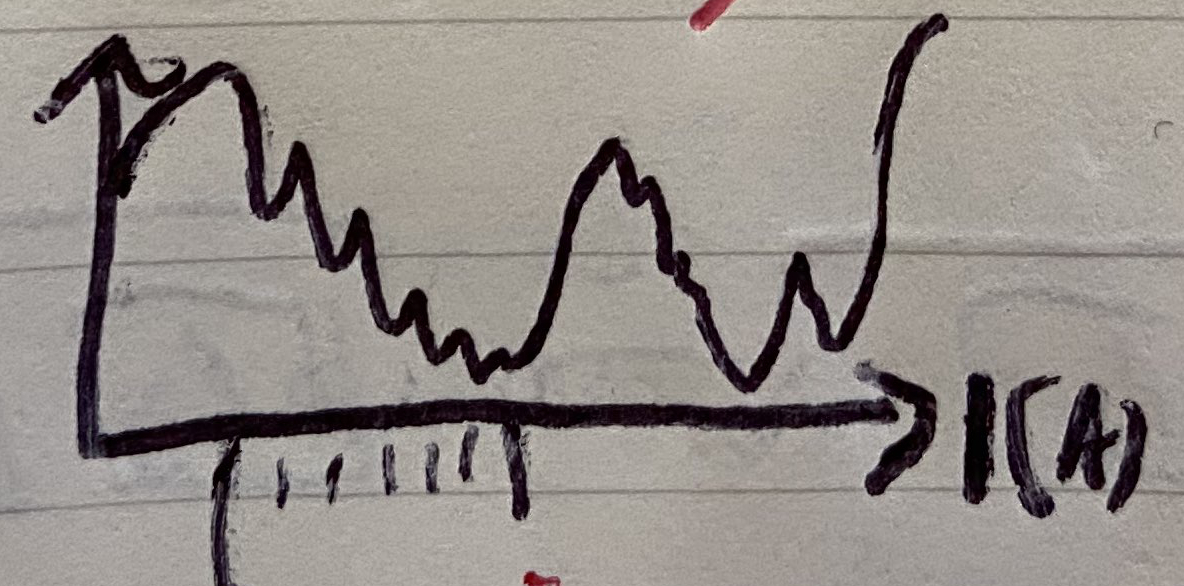
\includegraphics[keepaspectratio,width=2cm]{images/ivchar-draft}};
	\node (rg) at (4,0.5) {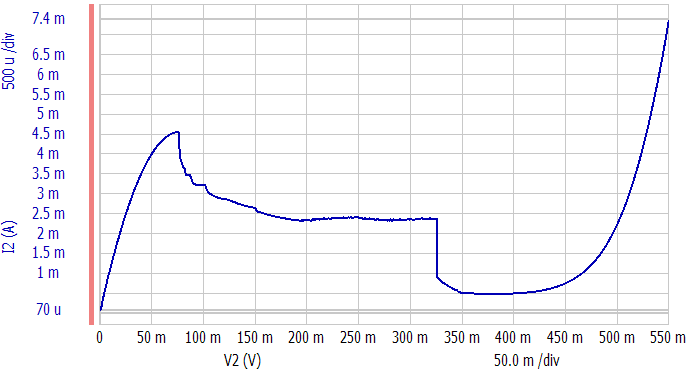
\includegraphics[keepaspectratio,width=3.5cm]{images/VI-png}};
	
	% Response
	\node[text=respcolour] (rval) at ($(rg) + (1,-1.3)$) {\texttt{u8}||\texttt{u8}||...||\texttt{u8}};
	\node[text=respcolour,font=\scriptsize] (rtext) at ($(rval) - (0,0.26)$) {Response: $m$ bits};
	
	\draw[color=respcolour, dashed] ($([xshift=-25]rg.south) + (0,0.4)$) -- ($([xshift=-25]rg.south) + (0,1.3)$);
	\draw[color=respcolour, dashed] ($([xshift=14]rg.south) + (0,0.4)$) -- ($([xshift=14]rg.south) + (0,1.3)$);
	\draw[color=respcolour, <->] ($([xshift=-25]rg.south) + (0,0.7)$) -- ($([xshift=14]rg.south) + (0,0.7)$);
	
	\draw[->, color=respcolour] ($(rg) - (2.45,0.5)$) to[out=90, in=180] (rg.west);
	
	\draw[->, color=respcolour] ($([xshift=14]rg.south) + (0,0.4)$) to[out=-90, in=90] ([xshift=20,yshift=5]rval);
	\draw[->, color=respcolour] ($([xshift=-25]rg.south) + (0,0.7)$) to[out=-90, in=100] ([xshift=-20,yshift=5]rval);
\end{tikzpicture}}
%			\end{figure}
%		\end{column}
%	\end{columns}
%\end{frame}

\section{Q3: Performance}

\begin{frame}{Setup}
	?? Baselines
	
	?? What Machines
	
	?? Waht NFs.
	
	?? WHy
\end{frame}

\begin{frame}{?? Results?}
	content...
\end{frame}

\begin{frame}{High-level}
	?? better at these things
	
	If you want more detailed data, please check out our paper
\end{frame}

%\begin{frame}{...What's next?}
%	\begin{itemize}
%		\item Currently measuring on RPi and NUC:
%		\begin{itemize}
%			\item Power, CPU use, ...
%			\item Latency (distribution), Throughput
%			\item Showing usefulness in relocating `expensive' NFs.
%		\end{itemize}
%		\item Working out the details on paper for control plane reconfiguration:
%		\begin{itemize}
%			\item eBPF ProgMaps, etc. allow atomic replacement.
%			\item Still need to codify details on chain \& map building to prevent inconsistencies.
%		\end{itemize}
%	\end{itemize}
%\end{frame}

\begin{frame}[standout]
	Takeaways:
	\begin{itemize}
		\item \alert{Cheap NFs}: SBCs for packet processing.
		\item \alert{Low-latency and fast}: XDP path for majority of traffic, early \& cheap anomaly checks, power savings.
		\item \alert{Secure}: PUFs for device, server, and function chain attestation.
		\item \alert{Easy to write}: \emph{native and XDP} portable NFs in Rust.
%		\item \emph{Ongoing work}: complex NFs, power + latency measures, better characterising PUF behaviour.
	\end{itemize}
	\alert{Questions?}\\
	{
		\scriptsize
		\vspace{2em}\faEnvelopeOpen{} \href{mailto:\myemail}{\nolinkurl{\myemail}}\\
		\vspace{-0.8em}	\small{\faGithub{} \href{https://github.com/\mygithub}{\mygithub} \hspace{0.5em} \faGlobe{} \url{\myurl}}
	}
	
	\begin{tikzpicture}[overlay, remember picture]
		%		\node[above right=0.8cm and 0.9cm of current page.south west] (esnet-logo) {
\includegraphics[width=2.75cm]{netlab-trim}};
		%		\node[right=1cm of esnet-logo] {\adjincludegraphics[height=2cm,trim={0 {.4\height} 0 {.05\height}},clip]{uofg}};
		\node[above left=0.2cm and 0.8cm of current page.south east] {
\includegraphics[width=2.75cm]{branding/netlab-fulllogo}};
		\node[above right=0.35cm and 0.8cm of current page.south west] {
\includegraphics[width=2.75cm]{branding/uofg-white}};
	\end{tikzpicture}
\end{frame}

%\begin{frame}[allowframebreaks]{References}
%	\printbibliography[heading=none]
%\end{frame}

\end{document}